This thesis centers on the modeling of passive daytime radiative cooling devices (PDRCs) utilizing the COMSOL Multiphysics™ software. While all objects with a temperature above absolute zero emit blackbody radiation, PDRCs are distinct in their ability to efficiently radiate heat in the mid-infrared range where the Earth's atmosphere is most transparent. This allows PDRCs to effectively transfer heat directly to the cold sink of outer space during daylight hours, without the need for input energy. Therefore, PDRCs hold the promise of addressing two significant challenges: the energy crisis and global warming.

% --------------- SECTION 1.1: COOLING IS CRITICAL ---------------

\section{Cooling is Critical}
Over the years, cooling has become more critical to humans due to global warming, rapid population growth and industrial development \cite{chen_passive_2022}. Various methods exist for cooling buildings, ranging from traditional practices, such as shading and solar orientation, to the use of electric fans. The most advanced approach is air conditioning (AC), encompassing systems that enhance indoor thermal comfort and air quality. While mechanical cooling techniques date back to the 19th century, widespread adoption of air conditioning began in the 1950s, driven by improved performance, affordability, and economic prosperity, primarily in the United States \cite{international_energy_agency_future_2018}.

Modern AC systems vary widely in size and cost, catering to individual rooms or entire buildings, with electricity being the predominant power source. Today, the largest concentration of cooling systems is found in urban areas, both in industrialized nations and emerging economies, reflecting the higher population density and greater demand for climate control in these regions \cite{international_energy_agency_future_2018}. 

Particularly in the realm of residential air conditioners (ACs), China emerges as the foremost market with a staggering sale of 41 million units. Following China, the USA, Japan and the European Union represent the subsequent largest markets for residential ACs. However, there is a significant uptick in sales within various emerging economies, notably in Asia (see Figure \ref{fig:sales_acs}).

Global sales of ACs have exhibited consistent growth in recent years. Over the period from 1990 to 2016, annual AC sales experienced a nearly fourfold increase, reaching 135 million units. In 2016, China emerged as the leading market in terms of AC capacity sales, totaling nearly 390 gigawatts (53 million units) \cite{international_energy_agency_future_2018}.

\begin{figure}
  \centering
  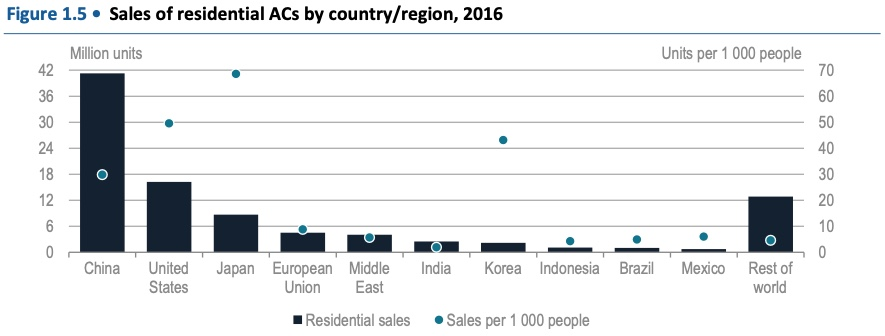
\includegraphics[width=0.8\textwidth]{Chapters/Figures/Sales of Residential ACs by Country or Region, 2016.jpg}
  \caption[Sales of Residential ACs by Country or Region, 2016]{Sales of Residential ACs by Country or Region, 2016. Source: \cite{international_energy_agency_future_2018}.}
  \label{fig:sales_acs}
\end{figure}

The growing demand for cooling is significantly influencing power systems, primarily due to the reliance on electricity-driven fans or air conditioners to meet cooling requirements. The escalating demand for air conditioning, in particular, not only elevates overall electricity consumption but also contributes to higher peak electricity loads. Additionally, the emission of greenhouse gases (GHGs) from ACs occurs through refrigerant leakage or improper disposal. It is noteworthy that these refrigerants are potent GHGs with adverse implications for climate change \cite{international_energy_agency_future_2018}.

Improving the efficiency of air conditioning systems (ACs) is pivotal in mitigating peak electricity demand, thereby resulting in decreased emissions and associated financial implications. Endeavors focused on enhancing cooling efficiency necessitate a thorough assessment of the comparative costs linked to diverse cooling technologies.

% --------------- SECTION 1.2: RADIATIVE COOLING ---------------

\section{Radiative Cooling}

\begin{figure}
  \centering
  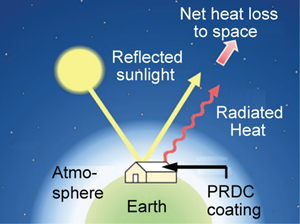
\includegraphics[width=0.5\textwidth]{Chapters/Figures/Schematic for Radiative Cooling.png}
  \caption[Schematic for Radiative Cooling] {Schematic for Radiative Cooling. Source: \cite{yang_passive_2020}}
  \label{fig:PDRC_Schematic}
\end{figure}

Objects with temperatures above absolute zero emit blackbody radiation, with a spectrum that depends on their temperature as governed by Planck's law. While the emitted radiation covers a range of wavelengths, it is not uniformly distributed across all wavelengths. Radiative passive cooling occurs when objects emit more radiation, particularly in the infrared spectrum, than the combined radiation they absorb, which includes both blackbody and solar radiation. Thus radiative passive cooling is an electricity-free method for cooling terrestrial entities \cite{yang_passive_2020}.

The heat emitted by these objects, which exceeds the heat they absorb, is transferred to outer space via thermal radiation, leveraging the substantial temperature difference between Earth (approximately 300 K) and outer space (approximately 3 K) (see Figure \ref{fig:PDRC_Schematic} for net heat loss to space). This process efficiently exchanges heat with the infinite cold reservoir of deep space, achieving cooling without any energy consumption \cite{chen_passive_2022}.

Passive radiative cooling can be realized even during the daytime, necessitating precise tuning of optical properties across a broad spectrum of wavelengths, from ultraviolet to mid-infrared (see Figure \ref{fig:ideal_PDRC_properties}). As a result, achieving effective passive daytime radiative cooling imposes stringent requirements on materials and structures to mitigate solar heating \cite{yang_passive_2020}:

\begin{enumerate} 
\item Minimal absorptivity ($\alpha$) approaching 0\% (equivalent to nearly 100\% reflectance, $R$) in the solar spectrum, ranging from 0.3–2.5 $\mu m$. This characteristic ensures that the surface absorbs minimal solar energy during daylight, thereby reducing the heat gained by the PDRC.
\item High thermal radiation in the atmospheric transparency window, with an emittance ($\varepsilon$) close to 1 within the long-wavelength infrared (LWIR) transmission window of the atmosphere ($\lambda$ = 8–13 $\mu m$). This range is significant due to the atmosphere's partial transparency and minimal infrared absorption by gas molecules in this spectrum.
\item An emittance ($\varepsilon$) close to 0 in other mid-infrared wavelengths, such as 5–8 $\mu m$ and those greater than 13 $\mu m$. This characteristic is crucial due to the atmosphere's opacity in these spectral ranges, and helps to minimize atmospheric blackbody radiation heating of the device due to its ability to reflect rather than absorb and re-emit infrared radiation in these wavelengths.
\end{enumerate}

% NB: Using [ht!] tells LaTeX to try to place the figure here, but if that's not possible, then at the top of the page, and the ! overrides LaTeX's internal parameters for deciding on figure placements. This gives you the best chance of having the figure appear right after your enumerated list, although it's not a guarantee because LaTeX might still decide to move the figure based on its page layout algorithms.

%Force the Figure Placement: While not generally recommended because it can disrupt the flow of text, using the float package with the [H] specifier instead of [ht!] can force the figure to appear exactly where it is defined in the code. Add \usepackage{float} in your preamble, and then:

\begin{figure}[H]
  \centering
  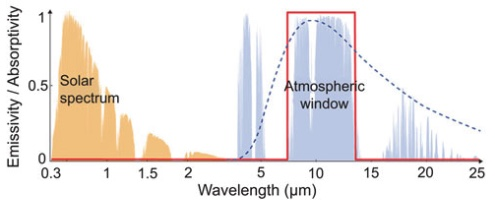
\includegraphics[width=0.7\textwidth]{Chapters/Figures/Ideal Optical Properties of a Radiative Cooling Surface.jpg}
  \caption[Ideal Optical Properties of a Radiative Cooling Surface]{Ideal Optical Properties of a Radiative Cooling Surface. Source: \cite{yang_passive_2020}}
  \label{fig:ideal_PDRC_properties}
\end{figure}

% --------------- SECTION 1.3: LITERATURE REVIEW ---------------

\section{Literature Review}
At the nexus of physics and technological advancement, Passive Daytime Radiative Cooling Devices (PDRCs) stand as a symbol of optimism amidst the challenges of global warming and the energy crisis. PDRCs are notable not just for their operational efficiency but also for their capacity to transform our approach to energy consumption and environmental conservation. While radiative cooling for nighttime use was established decades ago, only recently has there been significant progress in achieving cooling directly under sunlight, suggesting a promising upward trajectory for the technology's cooling capabilities.

\subsection{Historical Overview of Radiative Cooling.}
The concept of radiative cooling, hypothesized by French Engineer Félix Trombe in 1965, initially focused on nighttime cooling \cite{trombe_aspects_1965}. Significant strides have recently been made in achieving daytime cooling under direct sunlight, marking a pivotal advancement in the field. Trombe's collaboration at Montlouis Laboratory led to a cooling method that significantly reduced temperatures without insulation, leveraging a system that could cool by 14 to 30 degrees Celsius relative to the surroundings. This system involved a north-facing, slightly tilted facade with infrared-transparent panels and a selective radiator, optimizing both night and daytime cooling as seen in figure \ref{fig:Trombe_cooling_house} \cite{fortin_passive_2023}.

\begin{figure}[ht!]
  \centering
  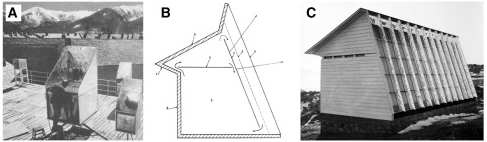
\includegraphics[width=0.4\textwidth]{Chapters/Figures/Trombe PDRC Structure.png}
  \caption[Experimental Cooling Container by Trombe et al.]{Experimental Cooling Container by Trombe and his team in Mont-Louis, France. (A) depicts the experimental cooling setup developed by Trombe's team in Mont-Louis. (B) presents a cross-sectional view of Trombe’s patented cold house design. (C) offers a northeast perspective of the cold house, showcasing its radiative cooling facade, a creation of Felix Trombe and his collaborators in 1963. Source: \cite{fortin_passive_2023}}
  \label{fig:Trombe_cooling_house}
\end{figure}
% TODO: Investigate whether this image, since it's small, can be made to "look more inline"

Building on Trombe's groundbreaking efforts, in 1975, Catalanotti and his team developed an experimental setup for daytime radiative cooling. This setup combined metals and TEDLAR (polyvinyl-fluoride plastic) to protect the cooling device from direct sunlight, although it was more effective for nighttime use \cite{bijarniya_review_2020}. This TEDLAR film, offering somewhat selective and high infrared (IR) absorption within the 9 to 13 $\mu m$ wavelength range, also absorbs IR significantly beyond 20 $\mu m$, impacting its selectivity and, consequently, the efficiency of radiative cooling. Despite this, they achieved a temperature decrease of 10 degrees Celsius below ambient under diffused sunlight. The primary drawback of using PVF polymer for daytime cooling is its substantial absorption in the solar spectrum \cite{hossain_radiative_2016}.

Further research explored the potential of thin films on aluminum substrates, with specific material compositions, such as coated thin solid film on an aluminum substrate with $\text{SiO}_6\text{N}_{0.2}$ and double layers of $\text{SiO}_2$ and $\text{SiO}_{0.25}\text{N}_{1.52}$, aimed at achieving selective emission. Despite these innovative approaches, effectively cooling during daylight remained a challenge \cite{bijarniya_review_2020}.

\subsection{Challenges with Material Selection.}
Ongoing advancements have aimed to enhance the cooling capabilities of radiative emitters, achieving notable success in nocturnal cooling. Yet, the reliance on both naturally sourced and synthetic polymers has imposed constraints. The absence of materials that combine high solar reflectivity with potent IR emission has hindered effective cooling under direct sunlight. Investigations into selective IR emitters, including polymer films, white pigmented paints, and SiO films, have encountered limitations due to their inadequate emissivity and the wide range of their IR absorption, which absorbs too much atmospheric radiation, thus failing to significantly lower temperatures below ambient conditions \cite{hossain_radiative_2016}.

\subsection{Exploration of Polymer Films and Pigmented Paints.}
Additional polymer films such as polyvinylchloride (PVC) and poly(4-methylpentene) (TPX) were evaluated for their potential in radiative cooling. However, their performance, particularly in terms of IR emissivity and selectivity within the crucial 8-13 $\mu m$ range, fell short when compared to PVF \cite{hossain_radiative_2016}.

Furthermore, investigations into pigmented paints, inorganic compounds, and gases capable of IR emission for nighttime cooling have shown promise. Specifically, white paint containing titanium dioxide (TiO$_2$), applied to aluminum plates, demonstrated notable cooling effects under clear sky conditions at night, despite less effectiveness under direct midday sun. This suggests pigmented paints might offer advantages for nocturnal cooling due to their application versatility on different substrates \cite{hossain_radiative_2016}.

% \subsection{The Role of Inorganic Materials in Radiative Cooling.}
The application of Silicon monoxide (SiO) films and other inorganic materials in radiative cooling technologies leverages their capacity for targeted infrared (IR) emission. These substances are recognized for their potential to efficiently radiate heat from surfaces, aiding in cooling processes. Nevertheless, their effectiveness is somewhat diminished by a narrow emission bandwidth, limiting the spectrum of IR radiation they can emit. This constraint may decrease the volume of heat dispersed into the environment, thereby affecting the device's cooling efficacy \cite{hossain_radiative_2016}.

\subsection{Innovations in Solar Reflectors and Convection Shields.}
Investigations into solar reflectors and IR-transparent materials for daytime cooling have proven effective in both reflecting solar radiation and facilitating IR emission. This capability is essential for daytime cooling to both prevent solar heat accumulation and promote surface heat release. However, maintaining this delicate balance during peak sunlight, when solar irradiance is most intense, presents a considerable challenge. Achieving the optimal mix of solar reflection to avoid overheating while ensuring adequate IR emission for cooling under direct sunlight is particularly complex \cite{hossain_radiative_2016}.

Beyond solar reflectors, convection shields significantly enhance a radiative cooler's effectiveness. In daytime operations, when a cooler's net radiative output exceeds its solar absorption, it can significantly lower temperatures beneath the ambient level, assuming convective heat gains are minimized. However, employing convection shields might not always be beneficial, as natural convection can help dissipate heat from the device. Yet, without direct sunlight, convection shields can markedly boost cooling efficiency to its maximum potential \cite{hossain_radiative_2016}.

\subsection{Photonic Devices and Microstructure Advances.}
The advancement in photonic-based radiative coolers represents a significant leap towards achieving efficient cooling directly under sunlight, allowing temperatures to fall below ambient levels. This innovative approach differs from traditional methods that rely on the natural optical characteristics of materials, as it harnesses engineered photonic properties in tandem with those natural characteristics to enhance cooling performance \cite{hossain_radiative_2016}.

Raman and colleagues conducted the inaugural experiment showcasing radiative cooling under direct sunlight with planar photonic structures (see figure \ref{fig:planar_photonic_device}), achieving a notable 4.9°C drop below ambient temperature. Their device, composed of seven layers alternating between hafnium oxide ($\text{HfO}_2$) and silicon dioxide ($\text{SiO}_2$) of varied thicknesses, utilized the upper thick layers for IR emission across the 8–13 $\mu m$ range. The lower, thinner layers on an aluminum-coated silicon wafer acted as a chirped 1D photonic crystal, reflecting up to 97\% of solar radiation \cite{raman_passive_2014}.

\begin{figure}[ht!]
  \centering
  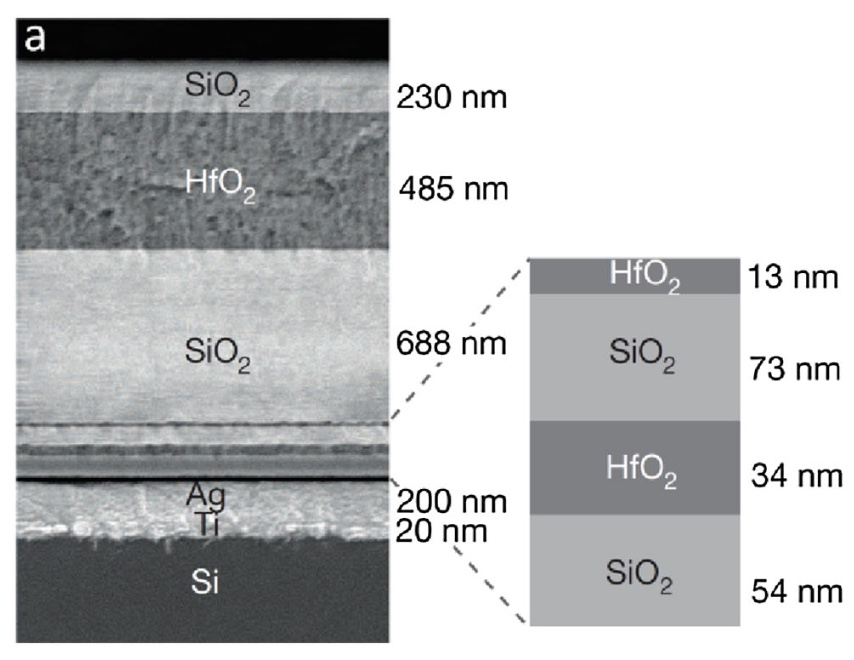
\includegraphics[width=0.4\textwidth]{Chapters/Figures/Planar Photonic Devices}
  \caption{Radiative cooling device consisting of seven layers of HfO2 and SiO2, whose thicknesses are defined by extensive numerical optimization (see Methods), on top of 200 nm of Ag, a 20-nm-thick Ti adhesion layer, and a 750-mm-thick, 200-mm-diameter Si wafer substrate. Source: \cite{raman_passive_2014}}
  \label{fig:planar_photonic_device}
\end{figure}

\subsection{Future Directions and Microfabrication Techniques.}
Metallic microstructures, like plasmonic structures and metallic photonic crystals, offer the potential for highly selective infrared (IR) emission. Achieving this selective emission across the full 8–13 $\mu m$ wavelength spectrum remains a challenge. Anisotropic metamaterials have shown promise, capable of strong and precise IR emission within this range. This technology could potentially enable cooling significantly below ambient temperatures by more than 10 degrees Celsius, illustrating the advanced capabilities and potential of these engineered materials for effective radiative cooling \cite{hossain_radiative_2016}.

Leveraging photonic microstructures for efficient cooling shows great promise but faces hurdles in practical application, particularly for daytime use where such radiators need to be paired with IR transparent solar reflectors to minimize solar absorption. This pairing, however, compromises the precise IR emission. Nonetheless, advancements in microfabrication techniques, like UV-nanoimprint lithography, offer improved prospects for scaling up production, potentially overcoming some of the challenges in deploying these technologies widely \cite{hossain_radiative_2016}.

% -- SECTION 1.4: PREVIOUS PROJECT WORK AND PROJECT GOALS ---

\section{Previous Project Work and Project Goals}
Research on PDRCs has been an ongoing project in the Hudgings lab. This thesis aims to build upon the work of Paul McKinley (class of 2022) and Genevieve diBari (class of 2023).

McKinley laid the groundwork by developing a rooftop testbed and the fabrication process for PDRCs (a process I plan to replicate after completing the modeling of various PDRC iterations on COMSOL). DiBari contributed by modeling PDRCs in Python and enhancing the initial outdoor testing setup.

For my thesis, the goal is to model different PDRC structures using COMSOL, exploring materials that could enhance the optical properties of an ideal PDRC device. This includes stacking materials of varying thicknesses and refractive indices on current PDRC models in the Hudgings lab to increase reflectivity ($R$). If time permits, promising PDRC models (with high $R$ and/or emissivity in the atmospheric window) will be fabricated after the modeling phase.
